\section{Transmitting the Data}\label{sec:transmitting_the_data}
TODO META\msmnote{fix}

\subsection{Data Structure for Communication}\label{sec:transmit}
\msmnote{rewrite, rm xml json. fair comp. w/ alt}
In \cref{sec:communication_methods} we decided to use WiFi Direct as our communication method.
In this section we determine a way to structure the data for network transmission. 
First we describe the different ways to structure the data, thereafter we choose one to implement.

\bigskip
The goal is for data transmission of various data types to have the least amount of overhead.
We have two types of data to transmit between the devices: music data, and commands.
Music data is parts of the song itself which is transmitted to the devices,
and the commands are the play, pause, stop, etc.\ commands sent from the master device to the slaves.
We need a method to send these two kinds of data between the devices in an efficient way,
to limit the amount of data transferred between the devices.
We desire to minimize two kinds of overhead: The size of the data, and the processing power used for serializing and deserializing.
To do this we want to use a well defined, mature, and well supported technology to do it.
Furthermore the data does not need to be human readable.

\subsubsection{The Data Structures}
To fulfill the requirements stated above, we have found two data structures: Protocol Buffers and Cap'n Proto. 

\paragraph{Protocol Buffers}
Protocol Buffers, also called Protobuf, are made by Google, and is a language and platform neutral extendible mechanism for serialized structured data.
Protobuf works by defining the way the data should be structured, this definition is then used to generate source code which can read and write the data to and from streams.\cite{protobuf}
Google supports protobufs for C++, C\#, Go, Java and Python, but nothing stops usage in other languages\cite{protobuf}.

Two supported versions of Protobuf exist: proto2 and proto3, where proto3 is the newest.
Proto3 have some changes from proto2, which makes it easier to implement in languages like Android Java, Objective C and Go.\cite{proto3}

\paragraph{Cap'n Proto}
Can'n Proto is, as protobuf, a data format with interchange in mind.
Like protobuf, Cap'n Proto works by defining the way data should be structured, which is then used to generate source code to manipulate the data in the desired language\cite{capnproto_schema}.
Cap'n Proto do not have any encoding and decoding which means that the data is sent directly without any conversion\cite{capnproto}.

Cap'n Proto supports many languages, i.e. C, C++, C\#, Go, Java, JavaScript, Lua, and more,
but it is only C++ which is officially supported, 
the rest of the languages are supported through third-party libraries and not reviewed by the author of Cap'n Proto\cite{capnproto_langs}. 
According to the roadmap of Cap'n Proto, there is still testing needed to be done and review of security\cite{capnproto_roadmap}.

\begin{table}
    \setlength{\tabcolsep}{10pt}
    \centering
    \begin{tabularx}{0.9\textwidth}{rXX}\toprule
        Data format & Pros                              & Cons \\\midrule
        Protobuf    & Tried and tested, \newline Official support for many languages & Not as fast as Cap'n Proto \\
        Cap'n Proto & Fast                              & Only official support for C++ \newline Still need some testing and review \\
    \end{tabularx}
    \caption{Pros and cons of protobuf and Cap'n Proto.}\label{tab:format_pros_cons}
\end{table}

\subsubsection{Choosing Data Transmission Medium}
Protobuf and Cap'n Proto are both language and platform neutral mechanism for serializing structured data.
Cap'n Proto is a bit faster than protobuf, but protobuf is more mature and official supports many languages. 
We value maturity high, since we need stability but speed is also important.

We feel that Cap'n Proto still need some development, so therefore we choose to use protobuf. 
More precisely, we will use proto3, since it is newer, less verbose and we expect it to be supported for a longer time period.

\subsection{Establishing a Persistent Socket}

After the slaves have discovered the master, they establish a persistent connection.
They are at this point part of the same WiFi Direct network, and the slave has just received the IP of the group owner.

When a device first starts its master mode, it launches a separate thread which opens a \code{ServerSocket} to accept incoming socket connections.
After accepting a connection it creates a \code{MessageConnection}, which is an abstraction for sending messages, which is run on a separate thread for each connection from the master to the slave, and vice versa.
The thread then continuously tries to read on the socket, to accept messages sent to it.

\subsubsection*{Creating our Protobufs}
As previously mentioned we decided to use protobufs to serialize our messages.
Just to be clear, a message is the entire payload sent from device to device, and the protobuf, is part of it.

We decided to use Wire Protocol Buffers\footnote{\url{https://github.com/square/wire}} made by Square to generate Java classes corresponding to our protobufs.
It is a mature library, and easily integrated into our app, it supports both proto2 and proto3, and generates builders for each of the classes it generates, making it easy to use.
The protobufs we use can be separated into three groups: meta-data, commands and data. \tnote{Tids ting går her under meta-data, er det fair?}
\begin{description}
    \item[Meta-data] \hfill \\
        Meta-data is information about the data, the data in this case is the audio data.
        The purpose of sending meta-data is twofold: we send it such that the clients can present it in their UI, and such that our audio player can be set up correctly.
        Our meta-data contains the following:
        \begin{itemize}
            \item Artist name
            \item Album name
            \item Song name
            \item Album art URL (An optional URL containing an image to be displayed)
            \item Song duration
            \item Media-info
        \end{itemize}
        Here the media-info contains the following information about the audio data (in the \ac{PCM} format). \tnote{Ref til Marcs afsnit om playback med begreberne}
        \begin{itemize}
            \item Sample rate
            \item Channels
            \item Encoding (bit depth per channel)
            \item Frame size
        \end{itemize}
    \item[Commands] \hfill \\
        Commands are used to change the playback on other devices.
        All commands contain a timestamp at which the given command should occur. \tnote{Evt. ref til core idea?}\tnnote{Ja, det synes jeg er en god idé.}
        In total we have the following commands:
        \begin{description}
            \item[PlayCommand]
                Used to start audio playback.
                Contains the location in the audio file to resume playback at, and the timestamp at which the playback should start.
            \item[PauseCommand]
                Used to pause audio playback.
                Much like the PlayCommand, it contains the location in the audio file at which the playback should pause, and the timestamp for when the pause should occur.
            \item[SeekCommand]
                Used to seek in the audio file, i.e. change which part of the audio file should be played.
                As the Play- and PauseCommands, it contains the location which the playback should change to, and the timestamp for when the change should occur.
            \item[SongChangeCommand]
                Used to change the audio file which should be played.
                Contains the meta-data for the file which will be changed to, and the timestamp for when the change should occur.
        \end{description}

    \item[Data] \hfill \\
        Lastly we have the data containing the audio itself, we call it: MusicData.
        MusicData contains a byte array, which is the \ac{PCM} audio data which will later be played, as explained in \tnote{ref til playback afsnittet}.
        As with the other messages, the MusicData contains a timestamp for when the audio data should be played.
\end{description}

\subsubsection{Sending the Messages}
When we designed the system we ran into a few issues, when it came to sending the messages.
Firstly we did not know which message we would be receiving next.
Secondly we did not know what length the next message would have.
This is a problem since, we would not know when to stop reading from the network connection, and start processing the data.
Additionally we would not know how to process the data.

To solve these issues, we add two integers to each message we send.
The first integer are assigned to each of the protobufs, such that the receiver knows which message it is.
The second integer is the length of the protobuf part of the message.
This is shown in \cref{fig:message_layout}.
This allow us to continue reading for exactly the amount of bytes the protobuf is.

Next the receiver can look up what decoder to use in order to deserialize the protobuf sent.
After the protobuf have been deserialized, we call the method registered to handle the given protobuf. \tnote{Vi skal måske forklare lidt mere om hvad det her indebærer?}

\begin{figure}[htb]
    \centering
    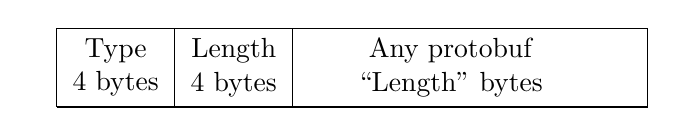
\begin{tikzpicture}[auto]
        \path[draw] (0,0) -- (0,1) -- (7.5,1) -- (7.5,0) -- (0,0) % Border
                        (1.5,0) -- (1.5,1) % Første streg (efter type)
                        (3.0,0) -- (3.0,1); % Anden streg (efter Length)

        \node[text width=2cm, align=center] at (0.75,0.5) {Type \\ 4 bytes};
        \node[text width=2cm, align=center] at (2.25,0.5) {Length \\ 4 bytes};
        \node[text width=4cm, align=center] at (5.0,0.5) {Any protobuf \\ ``Length'' bytes};
    \end{tikzpicture}
    \caption{The layout of any message we send.}
    \label{fig:message_layout}
\end{figure}
